\documentclass[11pt]{article}
\usepackage[margin=1in]{geometry}
\usepackage{graphicx}
\usepackage{booktabs}
\usepackage{amsmath}
\usepackage{microtype}
\usepackage[numbers,sort&compress]{natbib}
\usepackage[hidelinks]{hyperref}
\usepackage{caption}
\captionsetup{font=small,labelfont=bf}
\graphicspath{{figures/}}

\title{Leakage-controlled forecasts of full-season fantasy points and missed-time injury risk for the 2026 NFL season}
\author{Logan Hallee\\\small Synthyra}
\date{August 22, 2026}

\begin{document}
\maketitle

\begin{abstract}
We rank 951 fantasy-position NFL players for 2026 from public nflverse data using two chronologically audited models: a full-season ESPN full-PPR point forecast and a calibrated probability of a missed-time injury. Every input is a quantity from before the target season with recorded lineage, and historical candidate sets are built without target-season roster files. On the locked 2022--2025 audit the point forecast reaches mean within-position-season Spearman $\rho = 0.756$ (player-cluster 95\% interval 0.732 to 0.775) against 0.647 for prior-season points. The injury classifier reaches pooled 2022--2024 ROC AUC 0.749 (0.731 to 0.767) with calibration slope 1.02 at 24.7\% prevalence, against 0.677 for prior-year games alone. Participation and receiving usage dominate both feature rankings; injury history is a secondary signal. Two negative controls changed the protocol: target-permuted fits retained rank skill when training started before a 2017 change in roster coverage, and label-permuted fits retained pooled AUC because permutation preserves position prevalence. Adding literature-motivated usage shares and per-game rates did not improve either track.
\end{abstract}

\section{Objective}

For every fantasy-position player on the August 9, 2026 roster snapshot, predict the full regular-season ESPN full-PPR point total and the probability that the player misses time with an injury, then combine the two into a draft ranking. The two quantities are kept separate in every output so that a reader can apply a different risk preference.

\section{Data and leakage contract}

Inputs are nflverse Parquet releases frozen on August 10, 2026: weekly player statistics (1999--2025), weekly rosters (2002--2026), the player master, combine and draft tables, snap counts, and official injury reports (2009--2024) \citep{nflverse}. The target is the regular-season sum of player-game ESPN full-PPR points, including Week 18 since 2021, computed from raw counts with a versioned scoring profile; the nflverse fantasy-point column is never an input.

For a historical target season $t$ the candidate set is the union of players on a $t-1$ regular-season roster and $t$ draft or combine entrants. A candidate with no $t$ statistics keeps zero points. This avoids conditioning on eventual participation, which is unobservable at the August origin, and it is the main reason the rank metric is lower than numbers reported for cohorts that already know who played.

Every model column carries a lineage record naming its source table and season offset. Report-based injury history uses offsets of two or more seasons because the official feed ends after 2024; roster reserve history uses offsets of one or more. Target-season rosters, depth charts, status, projections, ADP, and nflverse composite efficiency metrics are excluded. Feature bundles reject any column whose lineage names an unlagged outcome source.

\section{Labels}

\textbf{Points.} Raw full-season points for QB, RB, WR, and TE. Kickers retain the earlier production forecast and are labeled low confidence because its audited gain over prior-season points had an interval that included zero.

\textbf{Missed-time injury.} A player-season is positive when the player is listed Out or Doubtful with a physical injury on an official regular-season report, or spends any regular-season roster week on an injury-compatible reserve list. Questionable-only and practice-only listings are negative; COVID, retired, did-not-report, left-squad, future, and suspension reserve codes are excluded. The label covers 2013--2024. Figure~\ref{fig:label} shows why the earlier any-designation label was replaced: its prevalence fell from about 45\% to 33\% when Probable left the reports in 2016, and it rewarded exposure. The missed-time label is stable at 22\% to 31\% from 2016.

\begin{figure}[t]
\centering
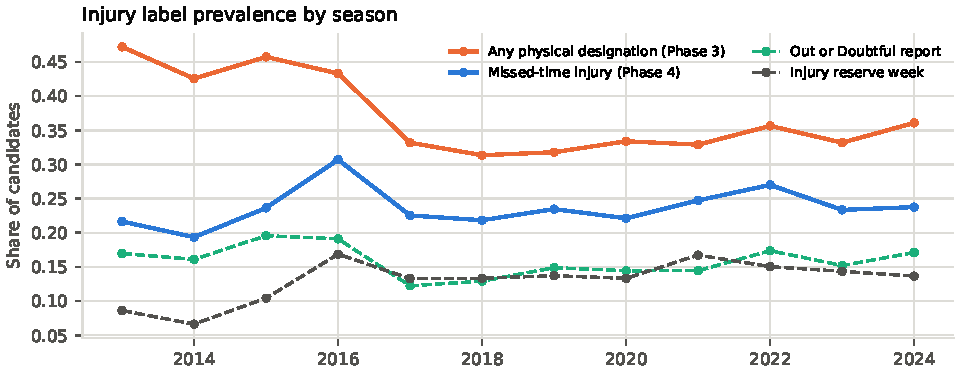
\includegraphics[width=\linewidth]{label_prevalence}
\caption{Prevalence of the two injury labels and of the missed-time components by target season among August-origin candidates.}
\label{fig:label}
\end{figure}

\section{Features}

The model vector has 512 columns in twelve families: cutoff metadata (age, experience, draft position, rookie flag), body and combine measurements, position indicators, lag-1 participation (games, roster weeks, snaps), lag-1 production counts and raw rates, lag-1 late-season trajectory, lags two to four of the same counts, missingness and history-availability indicators, report-based injury history at offsets two to five, and roster reserve weeks at offsets one to four. Rates are ratios of lagged raw counts; no imported composite enters.

Phase 5 added twelve literature-motivated columns, per-game rates and shares of the prior-season team's targets, carries, receptions, and attempts, following the predictor classes reported by published fantasy models and age-curve analyses \citep{smu2019,fourforfour2025,footballguys} and by injury-prediction reviews \citep{scoping2025}. They are evaluated in Section~\ref{sec:phase5}.

\section{Protocol}

\textbf{Folds.} Points models train on seasons from 2017 through $y-1$ and predict $y$. Injury models fit a base classifier through $y-2$, a sigmoid calibrator on $y-1$, and predict $y$. Development folds are 2019--2021 (points) and 2017--2021 (injury). Audits run once on 2022--2025 and 2022--2024. The plan, code, and input digests were recorded before fitting; three amendments are recorded with their triggers.

\textbf{Candidates and selection.} Points: the Phase 2 production model as reference, Extra Trees, histogram gradient boosting, and XGBoost on the extended inputs, and equal-weight blends. Selection keeps the best development Spearman within a 0.005 tolerance, preferring the reference, then fewer components, then lower MAE. A selected candidate is adopted only if its audit Spearman is not below the reference minus 0.005. Injury: age-position logistic, prior-games logistic, elastic net, two Extra Trees, and histogram gradient boosting; selection by AUC within 0.005, then log loss, then simplicity.

\textbf{Controls and uncertainty.} Five target or label permutations within season and position with refits; player-cluster bootstrap intervals (500 resamples); family ablation on development folds; held-out permutation importance; and an exposure diagnostic that restricts the injury audit to players with prior-year games.

\section{Results}

\subsection{Points}

\begin{table}[t]
\centering
\small
\caption{Locked 2022--2025 points audit, offense positions pooled (4{,}364 player-seasons).}
\label{tab:points}
\begin{tabular}{lccc}
\toprule
Candidate & Spearman & MAE & Top-$k$ recall \\
\midrule
Adopted Extra Trees, 512 inputs, trained from 2017 & \textbf{0.756} & \textbf{24.69} & 0.552 \\
Blend of Extra Trees and gradient boosting & 0.758 & 24.48 & 0.563 \\
Phase 2 production (228 inputs, trained from 2006) & 0.751 & 25.25 & 0.565 \\
Prior-season points & 0.647 & 27.18 & 0.555 \\
\bottomrule
\end{tabular}
\end{table}

Table~\ref{tab:points} and Figure~\ref{fig:points} give the audit. The adopted model's paired gain over Phase 2 is 0.005 (interval $-0.000$ to 0.009) and over prior-season points 0.109 (0.089 to 0.128). The blend scored slightly higher on the audit but was not selected on development folds, and the predeclared rule does not allow audit-driven choice.

\begin{figure}[t]
\centering
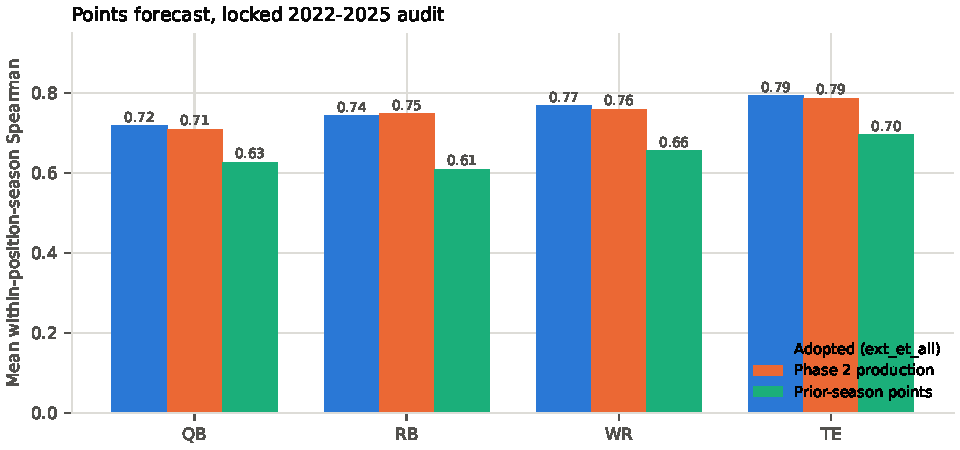
\includegraphics[width=0.85\linewidth]{points_audit_by_position}
\caption{Audit Spearman by position for the adopted model, the Phase 2 reference, and prior-season points.}
\label{fig:points}
\end{figure}

\subsection{Injury}

The selected classifier (300 Extra Trees, minimum leaf 50, 70\% features per split, balanced subsampling) reaches pooled audit AUC 0.749 (0.731 to 0.767), average precision 0.444, Brier 0.160, calibration intercept $-0.007$ and slope 1.019 (Figure~\ref{fig:injury}). Position AUC is 0.78 for QB and WR, 0.72 for RB, 0.71 for TE, and 0.60 for K. Within season and position the AUC is 0.683, which is the fairer statement of how well the model separates peers.

Participation is part of the signal: among players with at least eight prior-year games the audit AUC is 0.625 against 0.518 for prior-year games alone, so the model carries information beyond exposure, but less than the pooled number suggests. The same learner scores 0.868 on the earlier any-designation label, which confirms that label was easier because it was closer to a participation indicator.

\begin{figure}[t]
\centering
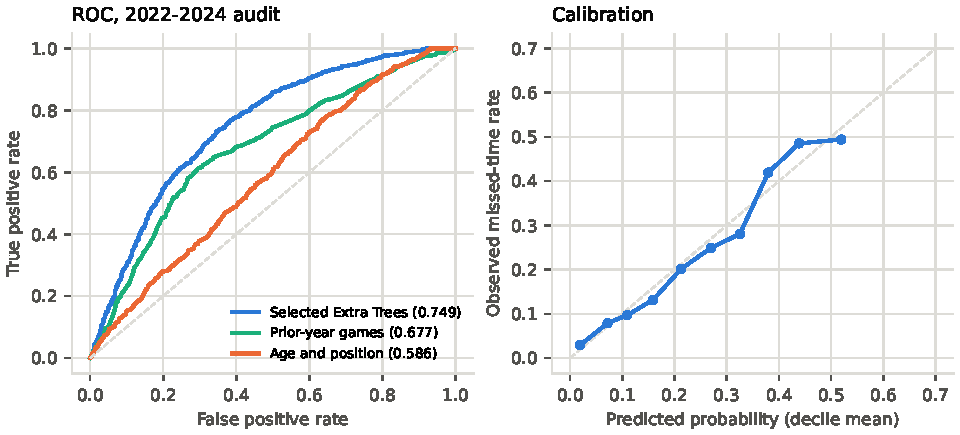
\includegraphics[width=\linewidth]{injury_roc_calibration}
\caption{Audit ROC against two baselines, and decile calibration of the selected classifier.}
\label{fig:injury}
\end{figure}

\subsection{Combination}

The position draft score is $100\,[(1-w)\,p + w\,(1-q)]$, where $p$ is the within-position percentile of projected points and $q$ the injury probability. The weight $w = 0.20$ is the largest grid value whose development-fold Spearman against realized points stayed within 0.005 of the best; on the audit it costs 0.004 Spearman. Figure~\ref{fig:weight} shows that no weight lowers the top-$k$ bust rate, so $w$ is a transparent risk preference rather than a backtested improvement. The cross-position page ranks by points over replacement (QB12, RB24, WR36, TE12, K12) scaled to the board maximum, with the health term centered on the position mean; without centering, four kickers led the board because low-exposure positions receive a blanket health bonus.

\begin{figure}[t]
\centering
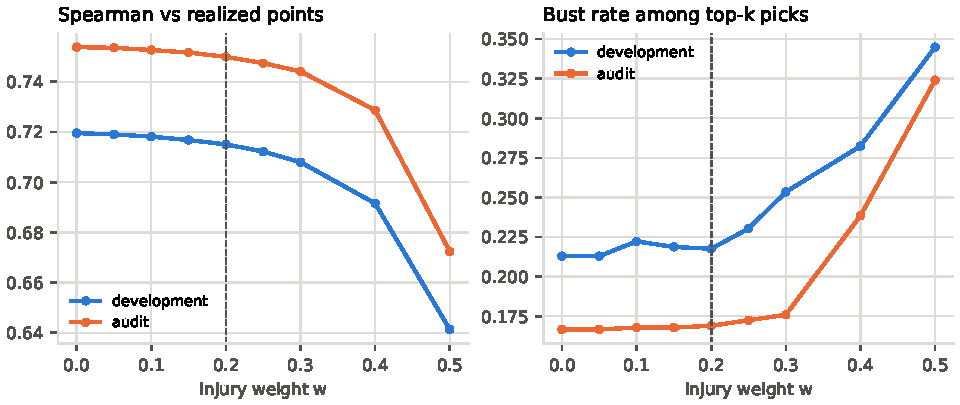
\includegraphics[width=\linewidth]{weight_tradeoff}
\caption{Rank accuracy against realized points and top-$k$ bust rate as the injury weight rises, on development and audit folds.}
\label{fig:weight}
\end{figure}

\subsection{Feature rankings}

Figure~\ref{fig:features} shows held-out permutation importance with the consensus rank over four evidence lines (permutation, univariate association, a mutual-information and random-forest panel, and FeatureRanker 3.0.4 \citep{featureranker}). Prior-year offensive snaps, games, receptions, targets, and yards after catch lead both tracks; draft position and its missingness matter for points; the first injury-history column appears at consensus rank 44. Figure~\ref{fig:ablation} gives the family ablation: removing age, experience, and draft costs the most points Spearman (0.0095), and removing prior-year participation costs the most injury AUC (0.0022). Most families are redundant with one another, which is why single-feature importances are small.

\begin{figure}[t]
\centering
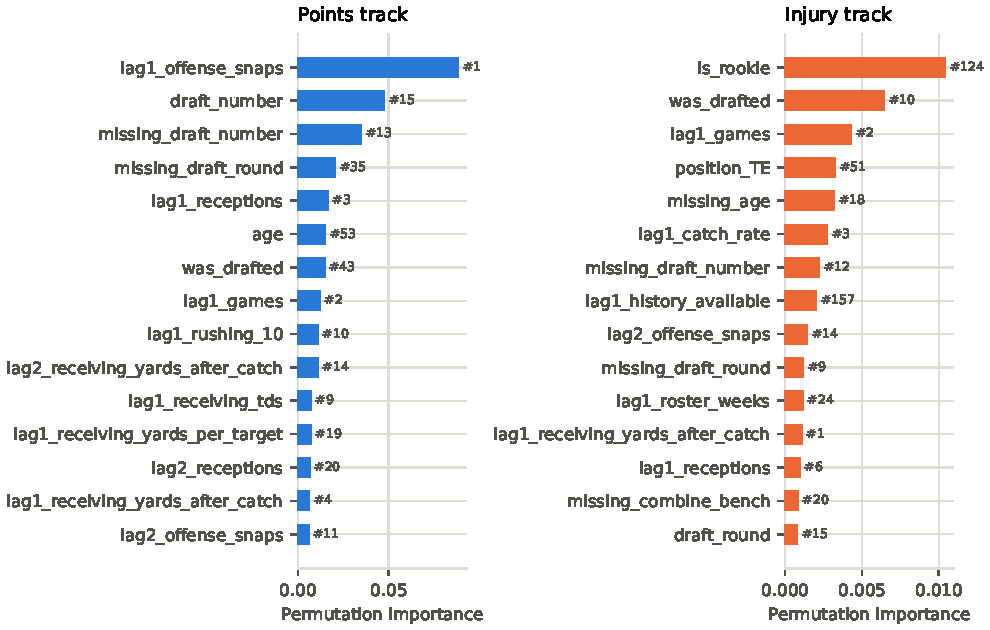
\includegraphics[width=\linewidth]{feature_importance}
\caption{Top 15 features per track by held-out permutation importance, annotated with the four-line consensus rank.}
\label{fig:features}
\end{figure}

\begin{figure}[t]
\centering
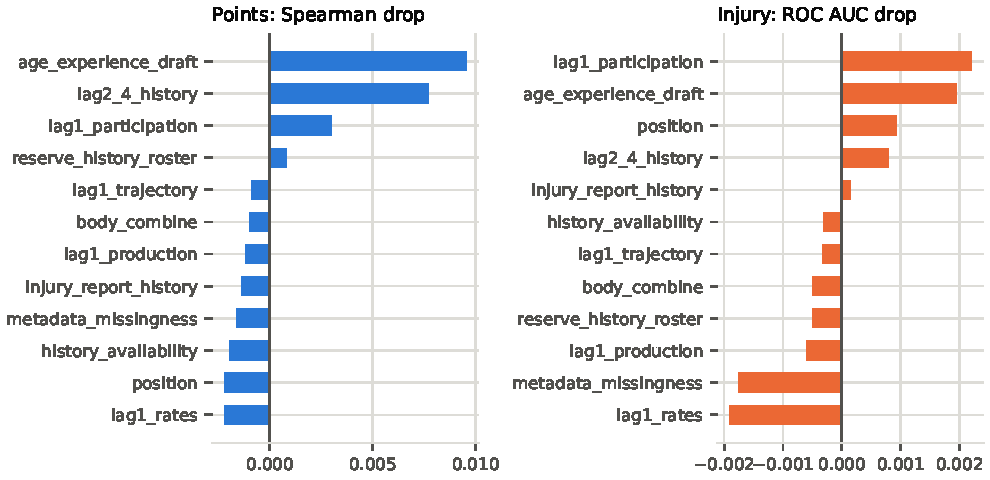
\includegraphics[width=\linewidth]{family_ablation}
\caption{Development-fold metric drop when one feature family is removed and the model is refit.}
\label{fig:ablation}
\end{figure}

\section{Negative controls that changed the protocol}

Figure~\ref{fig:null} summarizes both findings. First, with training from 2013 the target-permuted Extra Trees retained mean Spearman 0.108 on 2019--2021, above the 0.05 gate. Mean target points per season fall from about 57 to 40 in 2017 when the weekly roster files widen their coverage, and a model fitted to permuted targets can still learn era-proxy features that carry within-season structure. Training from 2017 moves the null to 0.027 with real skill unchanged (0.714 against 0.720). The window was amended, the full protocol was rerun, and the pre-amendment run is recorded in the plan; its audit had already been computed, which is one reason the audits are described as not analyst-blinded. Second, label-permuted injury fits retain pooled AUC 0.53 because the within-position permutation preserves position prevalence (kickers 17\%, running backs 26\%); within season and position the null is 0.478. Both controls pass after the amendment, and the audited skill exceeds the null by an order of magnitude.

\begin{figure}[t]
\centering
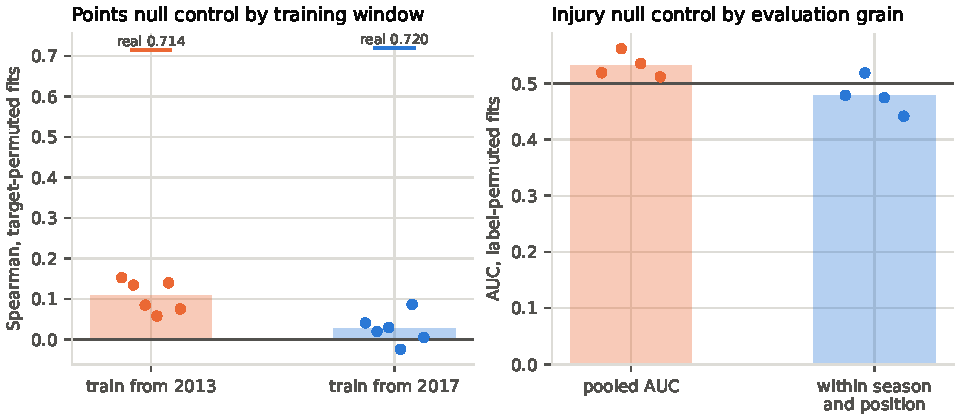
\includegraphics[width=\linewidth]{null_controls}
\caption{Left: Spearman of target-permuted points fits by training window, with real skill marked. Right: AUC of label-permuted injury fits pooled and within season and position.}
\label{fig:null}
\end{figure}

\section{Usage-share features}
\label{sec:phase5}

Under the identical protocol with the Phase 4 model as the reference, the twelve usage columns produced development Spearman 0.7197 against 0.7196 and audit 0.7548 against 0.7557; the best blend reached 0.7574, inside tolerance, so the rule retained the reference. Injury audit AUC was 0.749 against 0.749. The published predictor classes are therefore already represented by the raw lagged counts and their ratios in this feature set.

\section{Limitations}

The audits are chronological and procedure-locked but not analyst-blinded; earlier phases examined the same seasons. Historical August rosters are reconstructed from the prior season. The injury label records observed absence events, so players who play through injuries or leave the league are negatives. Point intervals in the workbook are empirical residual percentiles from the audit seasons, not calibrated predictive intervals. The replacement-level cutoffs and the injury weight are league-format and preference assumptions. The 2026 season is the prospective test.

\bibliographystyle{plainnat}
\bibliography{references}

\end{document}
